\documentclass[aspectratio=169]{beamer} % O parâmetro aspectratio com valar 16:9 deixa o slide em widescreen

\usepackage[brazil]{babel}
\usepackage[utf8]{inputenc}
\usepackage[T1]{fontenc}

\usetheme{Madrid}
\setbeamertemplate{navigation symbols}{}

\title[Informática]{Informática}

\author[Diego S. C. Nascimento]{Diego Silveira Costa Nascimento}

\institute[IFRN]{
Instituto Federal de Educação, Ciência e Tecnologia do Rio Grande do Norte\\
diego.nascimento@ifrn.edu.br
}

\date[\today]{\today}

\begin{document}

\begin{frame}[plain]
	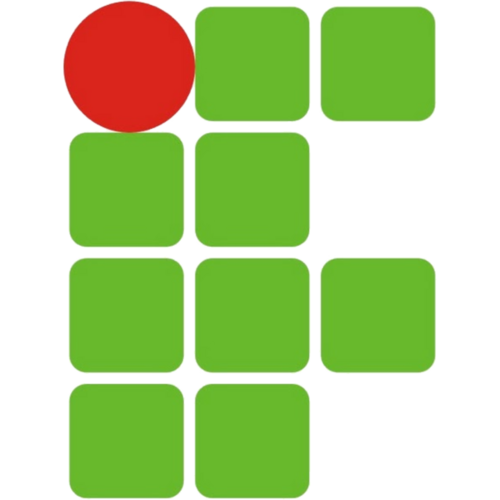
\includegraphics[scale=0.2]{img/IFRN}
	\titlepage
\end{frame}

\logo{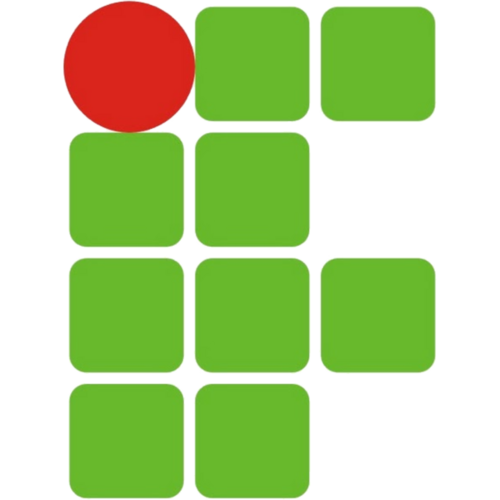
\includegraphics[scale=0.1]{img/IFRN}}

\begin{frame}
	\frametitle{Ementa do Curso}
  	\tableofcontents
\end{frame}

\AtBeginSection[]{
	\begin{frame}
		\frametitle{Ementa}
		\tableofcontents[currentsection]
	\end{frame}
}

\section{Introdução}

\begin{frame}
	\frametitle{História}
	
	\begin{itemize}
		\item Parte da evolução aconteceu ao mero acaso;
		\item A outra parte se deve a poucos homens que observaram os problemas cotidianos e tentaram encontrar um solução;
		\item Cada época apresentada seus principais pensadores, inventores e pessoas de diversos níveis de conhecimento;
		\item Para que uma invenção pudesse ser conhecida, havia uma demora de anos ou décadas; e
		\item O intervalo de conhecimento e de descobertas da humanidade vai diminuindo consideravelmente.
	\end{itemize}
\end{frame}

\begin{frame}
	\frametitle{As mãos}
	
	\begin{itemize}
		\item Primeira forma de mostrar uma quantidade; 
		\item Serviram como instrumentos de comparação; e
		\item Provavelmente aí está a origem do nosso sistema de numeração de base decimal (10 dedos).
	\end{itemize}\vfill
	
	\begin{exampleblock}{Ilustra\c cão}
		\begin{center}
			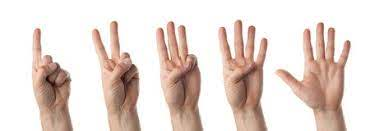
\includegraphics[scale=0.5]{img/dedos}
		\end{center}
	\end{exampleblock}
\end{frame}

\begin{frame}
	\frametitle{Objetos}
	
	\begin{itemize}
		\item Em latim, pedrinha se escreve \textit{calculu}.
	\end{itemize}\vfill
	
	\begin{exampleblock}{Ilustra\c cão}
		\begin{center}
			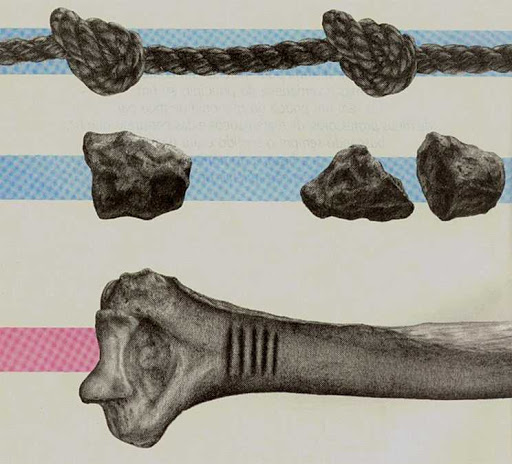
\includegraphics[scale=0.2]{img/objetos}
		\end{center}
	\end{exampleblock}
\end{frame}

\begin{frame}
	\frametitle{Ábaco}
	
	\begin{itemize}
		\item Provavelmente inventado na China (Dinastia de Yuan); e
		\item É o primeiro instrumento de calcular que se tem conhecimento.
	\end{itemize}\vfill
	
	\begin{exampleblock}{Ilustra\c cão}
		\begin{center}
			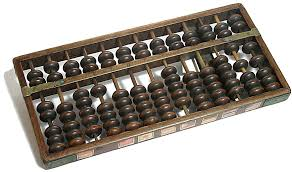
\includegraphics[scale=0.5]{img/abaco}
		\end{center}
	\end{exampleblock}
\end{frame}

\begin{frame}
	\frametitle{Ossos de Napier}
	
	\begin{itemize}
		\item John Napier foi um matemático escocês;
		\item Desenvolveu um conjunto de noves bastões chamados de Ossos de Napier; e
		\item Eram usados para multiplicar e dividir números elevados.
	\end{itemize}\vfill
	
	\begin{exampleblock}{Ilustra\c cão}
		\begin{center}
			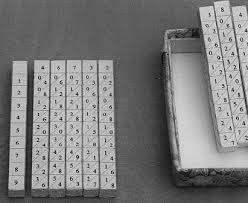
\includegraphics[scale=0.5]{img/ossos_napier}
		\end{center}
	\end{exampleblock}
\end{frame}

\begin{frame}
	\frametitle{Pascalina}
	
	\begin{itemize}
		\item Blaise Pascal, em 1642, inventou a primeira máquina de somar;
		\item Executava operações aritméticas quando se giravam os discos interligados; e
		\item Foi a precursora das calculadoras mecânicas.
	\end{itemize}\vfill
	
	\begin{exampleblock}{Ilustra\c cão}
		\begin{center}
			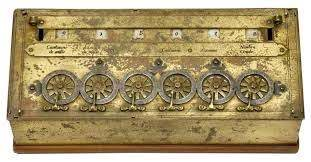
\includegraphics[scale=0.5]{img/pascalina}
		\end{center}
	\end{exampleblock}
\end{frame}

\begin{frame}
	\frametitle{Máquina de Leibniz}
	
	\begin{itemize}
		\item O alemão Gottfried Wilhelm Leibniz, em 1671, inventou uma máquina muito parecida com a Pascalina;
		\item Efetuava cálculos de multiplicação e divisão; e
		\item Se tornou a antecessora direta das calculadoras manuais.
	\end{itemize}\vfill
	
	\begin{exampleblock}{Ilustra\c cão}
		\begin{center}
			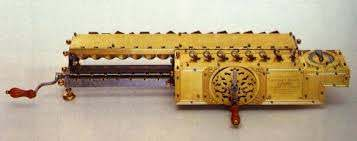
\includegraphics[scale=0.5]{img/maquina_leibniz}
		\end{center}
	\end{exampleblock}
\end{frame}

\begin{frame}
	\frametitle{Tear mecânico de Jacquard}
	
	\begin{itemize}
		\item Joseph-Marie Jacquard, em 1801, inventou um tear mecânico;
		\item Utilizava cartões perfurados;
		\item Fazia combinações de desenhos mais sofisticadas; e
		\item Cartões perfurados seriam posteriormente usados para projetar máquinas de calcular.
	\end{itemize}\vfill
	
	\begin{exampleblock}{Ilustra\c cão}
		\begin{center}
			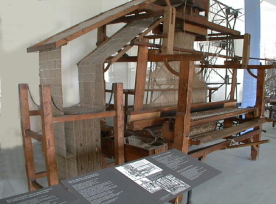
\includegraphics[scale=0.5]{img/tear_jacquard}
		\end{center}
	\end{exampleblock}
\end{frame}

\begin{frame}
	\frametitle{Máquina diferencial}
	
	\begin{itemize}
		\item Charles Babbage é conhecido como o \structure{Pai da Computação};
		\item Em 1822, desenvolveu a máquina diferencial de Babbage; 
		\item Permitia cálculos de funções trigonométricas e logarítmicas; e 
		\item Utilizava os cartões de Jacquard.
	\end{itemize}\vfill
	
	\begin{exampleblock}{Ilustra\c cão}
		\begin{center}
			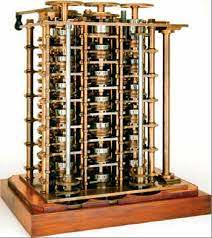
\includegraphics[scale=0.5]{img/maquina_diferencial}
		\end{center}
	\end{exampleblock}
\end{frame}

\begin{frame}
	\frametitle{Máquina analítica}
	
	\begin{itemize}
		\item Charles Babbage, em 1834, desenvolveu a máquina analítica;
		\item Permitia somar, dividir, subtrair e multiplicar;
		\item Armazenava dados em memória de até 1000 números de 50 dígitos; e 
		\item Imprimia resultados;
	\end{itemize}\vfill
	
	\begin{exampleblock}{Ilustra\c cão}
		\begin{center}
			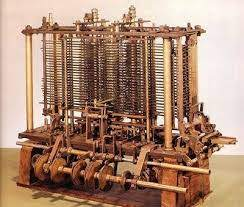
\includegraphics[scale=0.5]{img/maquina_analitica}
		\end{center}
	\end{exampleblock}
\end{frame}

\begin{frame}
	\frametitle{Tabulador de Hollerith}
	
	\begin{itemize}
		\item Desenvolvida para o censo dos EUA;
		\item  Hermann Hollerith percebeu que só terminaria de apurar os dados do censo quando já seria o tempo de se efetuar novo censo;
		\item Integrou a ideia dos cartões de Jacquard e do conceito de impulsos elétricos para a transmissão de dados;
		\item Tabulating Machine Company (1896); e
		\item Em 1924, tornou-se a International Business Machines Corporation – IBM.
	\end{itemize}\vfill
	
	\begin{exampleblock}{Ilustra\c cão}
		\begin{center}
			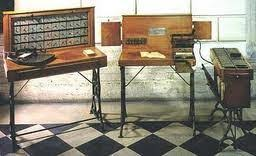
\includegraphics[scale=0.5]{img/tabulador_hollerith}
		\end{center}
	\end{exampleblock}
\end{frame}

\begin{frame}
	\frametitle{Computômetro}
	
	\begin{itemize}
		\item Foi desenvolvido por  Dorr Eugene Felt em 1887; e
		\item Primeira máquina com teclado para somar e imprimir.
	\end{itemize}\vfill
	
	\begin{exampleblock}{Ilustra\c cão}
		\begin{center}
			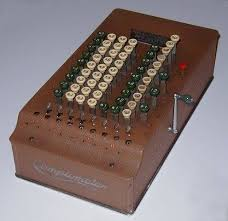
\includegraphics[scale=0.5]{img/computometro}
		\end{center}
	\end{exampleblock}
\end{frame}

\begin{frame}
	\frametitle{Mark I}
	
	\begin{itemize}
		\item Foi desenvolvido por Howard Aiken em 1937;
		\item Foi o primeiro computador eletromecânico, construído na Universidade de Harvard;
		\item Ajuda financeira da IBM: US\$ 500.000,00;
		\item Controlado por programa e usava o sistema decimal;
		\item Cerca de 15m de comprimento e 2,5m de altura; e
		\item Realizava uma soma em 0,3s, uma multiplicação em 0,4s e uma divisão em cerca de 10s.
	\end{itemize}\vfill
	
	\begin{exampleblock}{Ilustra\c cão}
		\begin{center}
			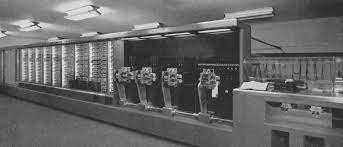
\includegraphics[scale=0.5]{img/marki}
		\end{center}
	\end{exampleblock}
\end{frame}

\begin{frame}
	\frametitle{Série Z1, Z2, Z3, Z4 e Z5}
	
	\begin{itemize}
		\item Desenvolvido pelo engenheiro alemão Konrad Zuse;
		\item  Computador construído à base de relés; e
		\item Os cálculos eram baseados em aritmética binária.
	\end{itemize}\vfill
	
	\begin{exampleblock}{Ilustra\c cão}
		\begin{center}
			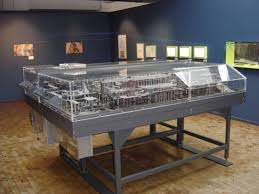
\includegraphics[scale=0.5]{img/z1}
		\end{center}
	\end{exampleblock}
\end{frame}

\begin{frame}
	\frametitle{Colossus}
	
	\begin{itemize}
		\item Projetado pelo matemático britânico Alan Turing em 1944;
		\item Usado para decifrar os códigos de Hitler na Segunda Gerra Mundial; e
		\item Ao invés de relés eletromecânicos, usava 2.000 válvulas eletrônicas.
	\end{itemize}\vfill
	
	\begin{exampleblock}{Ilustra\c cão}
		\begin{center}
			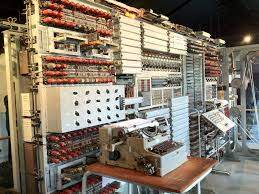
\includegraphics[scale=0.5]{img/colossus}
		\end{center}
	\end{exampleblock}
\end{frame}

\begin{frame}
	\frametitle{ENIAC}
	
	\begin{itemize}
		\item John Eckert e John Mauchly construíram o Eletronic Numerical Integrator and Calculator (ENIAC) em 1946;
		\item Primeiro computador eletrônico digital de propósito geral;
		\item Consumo cerca de 200 KW de potência;
		\item Memória podia registrar até 20 números de 10 dígitos cada um; e 
		\item Fazia 5.000 adições e 360 multiplicações por segundo.
	\end{itemize}\vfill
	
	\begin{exampleblock}{Ilustra\c cão}
		\begin{center}
			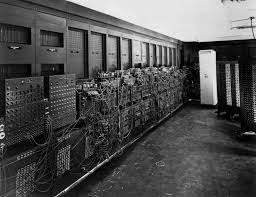
\includegraphics[scale=0.4]{img/eniac}
		\end{center}
	\end{exampleblock}
\end{frame}

\begin{frame}
	\frametitle{UNIVAC}
	
	\begin{itemize}
		\item John Eckert e John Mauchly construíram o Universal Automatic Computer (UNIVAC) em 1951;
		\item Primeiro computador comercial entregue a um cliente; e
		\item Era um ENIAC modificado.
	\end{itemize}\vfill
	
	\begin{exampleblock}{Ilustra\c cão}
		\begin{center}
			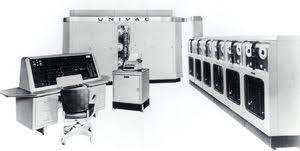
\includegraphics[scale=0.5]{img/univac}
		\end{center}
	\end{exampleblock}
\end{frame}

\begin{frame}
	\frametitle{TRADIC}
	
	\begin{itemize}
		\item Jean Howard Felker  construiu o Transistor Digital Computer (TRADIC) em 1954; e
		\item Primeiro computador 100\% transistorizado.
	\end{itemize}\vfill
	
	\begin{exampleblock}{Ilustra\c cão}
		\begin{center}
			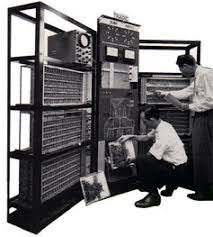
\includegraphics[scale=0.5]{img/tradic}
		\end{center}
	\end{exampleblock}
\end{frame}

\begin{frame}
	\frametitle{IBM 1401}
	
	\begin{itemize}
		\item Desenvolvido em 1959; 
		\item Totalmente transistorizado;
		\item Possuía capacidade de memória base de 4.096 bytes operando em ciclos de memória de 12 microssegundos; e
		\item Utilizado em vários seguimentos de mercados, principalmente por bancos.
	\end{itemize}\vfill
	
	\begin{exampleblock}{Ilustra\c cão}
		\begin{center}
			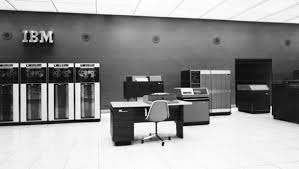
\includegraphics[scale=0.5]{img/ibm1401}
		\end{center}
	\end{exampleblock}
\end{frame}

\begin{frame}
	\frametitle{IBM System 360}
	
	\begin{itemize}
		\item Lançado em 1964; 
		\item Utilizava circuitos integrados; e 
		\item Constituia uma família de mainframes.
	\end{itemize}\vfill
	
	\begin{exampleblock}{Ilustra\c cão}
		\begin{center}
			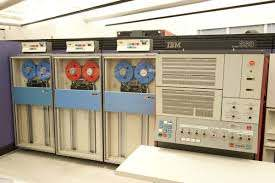
\includegraphics[scale=0.5]{img/ibm360}
		\end{center}
	\end{exampleblock}
\end{frame}

\begin{frame}
	\frametitle{Apple I}
	
	\begin{itemize}
		\item Steve Jobs e Steve Wozniak construíram o Apple I em 1976;
		\item Era uma placa de circuito impresso totalmente montada, contendo cerca de 30 chips;
		\item Um microprocessador MOS 6502 de 1 MHz;
		\item 4 k de memória;
		\item Tinham de acrescentar um gabinete, fonte de energia, teclado e monitor; e
		\item Permitia placa de expansão, contendo uma interface para cassetes, utilizados no armazenamento dos dados e programas.
	\end{itemize}\vfill
	
	\begin{exampleblock}{Ilustra\c cão}
		\begin{center}
			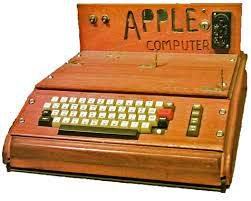
\includegraphics[scale=0.4]{img/apple1}
		\end{center}	
	\end{exampleblock}
\end{frame}

\begin{frame}
	\frametitle{Apple II}
	
	\begin{itemize}
		\item Lançado em 1977;
		\item Foi um sucesso no mercado de microcomputadores; 
		\item Possuia monitor e teclado juntos; e
		\item Memória RAM de 16 KB.
	\end{itemize}\vfill
	
	\begin{exampleblock}{Ilustra\c cão}
		\begin{center}
			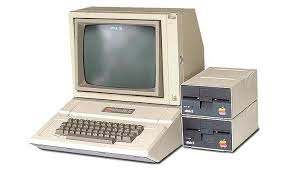
\includegraphics[scale=0.4]{img/apple2}
		\end{center}	
	\end{exampleblock}
\end{frame}

\begin{frame}
	\frametitle{IBM PC}
	
	\begin{itemize}
		\item Anunciado em 1981;
		\item Usava processador Intel 8086 de 4.77 MHz; e
		\item Possuia disquete com capacidade de armazenamento de 160 KB.
	\end{itemize}\vfill
	
	\begin{exampleblock}{Ilustra\c cão}
		\begin{center}
			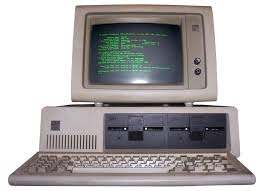
\includegraphics[scale=0.4]{img/ibmpc}
		\end{center}		
	\end{exampleblock}
\end{frame}

\begin{frame}
	\frametitle{Compaq Portable}
	
	\begin{itemize}
		\item Lançado em 1982
		\item Usava processador Intel 80286; 
		\item Possuia memória RAM de 16 MB; e 
		\item Pesava em torno de 11 kg.
	\end{itemize}\vfill
	
	\begin{exampleblock}{Ilustra\c cão}
		\begin{center}
			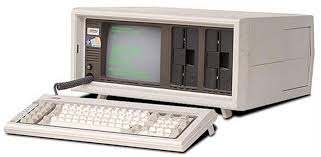
\includegraphics[scale=0.4]{img/compac_portable}
		\end{center}			
	\end{exampleblock}
\end{frame}

\begin{frame}
	\frametitle{Lisa}
	
	\begin{itemize}
		\item Lança em 1982 pela Apple;
		\item Trazia um mouse;
		\item Possuia interface gráfica;
		\item Disquetes com capacidade de armazenamento de 260 KB; e 
		\item Trazia um disco rígido (winchester) com capacidade de 10 MB de armazenamento.
	\end{itemize}\vfill
	
	\begin{exampleblock}{Ilustra\c cão}
		\begin{center}
			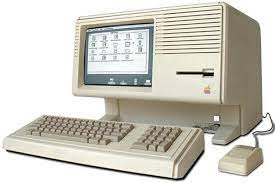
\includegraphics[scale=0.4]{img/lisa}
		\end{center}			
	\end{exampleblock}
\end{frame}

\begin{frame}
	\frametitle{Macintosh}
	
	\begin{itemize}
		\item Lança em 1984 pela Apple;
		\item  Nome inspirado em uma espécie de maçã canadense; e
		\item Possuia interface gráfica mais amigável.
	\end{itemize}\vfill
	
	\begin{exampleblock}{Ilustra\c cão}
		\begin{center}
			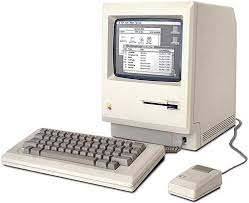
\includegraphics[scale=0.4]{img/macintosh}
		\end{center}			
	\end{exampleblock}
\end{frame}

\begin{frame}
	\frametitle{Tecnologias atuais}
	
	\begin{itemize}
		\item Desktop;
		\item Notebook;
		\item Smartphone;
		\item Tablet;
		\item Smartwatch; e
		\item Smartglass.
	\end{itemize}
\end{frame}

\end{document}